\section{Gewöhnliche Differentialgleichungen (DGL)}

Kurz \textcolor{blue}{DGL}, die Veränderung ($y'(x)$) einer Funktion an einem Punkt ist abhängig vom Wert
der Funktion selbst
$$\frac{dy}{dx} = f(x, y(x))$$

Eine solche gleichung nennt man gewöhnliche Differentialgleichung 1. Ordnung
(1. Ordnung weil nur die erste Ableitung vorkommt, engl. ODE = Ordinary
Differential Equation)



\subsection{gewöhnliche Differentialgleichung $n$-ter Ordnung}

Eine Gleichung in der Ableitungen einer unbekannten Funktion $y = y(x)$ bis zur $n$-ten
Ordnung auftreten.

Explizite Form:
{\Large
$$y^{(n)}(x) = f(x, y(x), y'(x), ..., y^{(n-1)}(x))$$
}

Beispiel:
$$y''(x) = y'(x)^3 * y(x) + cos(x) = f(x, y(x), y'(x))$$

Gesucht sind Lösungen $y : [a,b] \to \R = y(x)$ dieser Gleichung wobei die Lösungen
$y$ auf einem Interval $[a,b]$ definiert sind.



\subsection{Anfangswertproblem (AWP)}

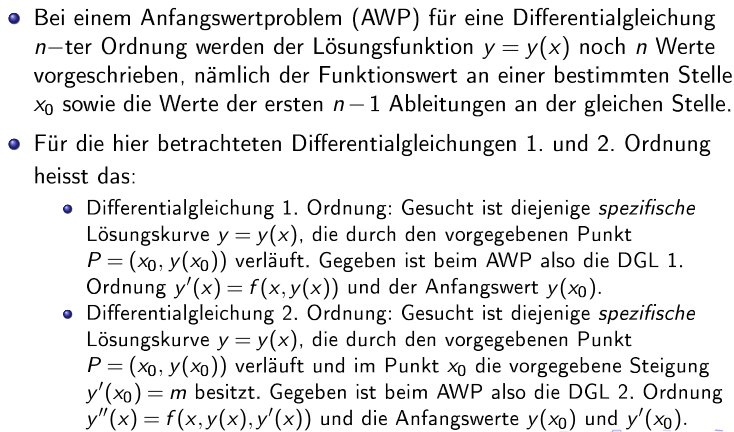
\includegraphics[scale=0.32]{diff-awp}












\subsection{Richtungsfelder (1. Ordnung)}

Die verschiedenen Lösungen einer DGL 1. Ordnung lassen sich als Richtungsfeld
darstellen. Hierbei wird in jedem Punkt $(x,y(x))$ die Steigung $y'(x) = f(x, y(x))$
als Pfeil eingezeichnet.

In dem man diesen Pfeilen entlang einer Kurve ''folgt'' hat man eine
spezifische Lösung.






\section{Einzelschrittverfahren}

\begin{itemize}
	\item gesucht: Funktion $y : [a, b] \to \R$
	\item Anfangsbediung $y(a) = y_0$
	\item Schrittweite $h = \frac{b-a}{n}$ wählen und Intervall $[a,b]$
	      mit $n+1$ Gittsterstellen $x_i = a + i*h \; | \; i = 0,1,...,n$
	      aufteilen
	\item Ziel: für alle Gitterstellen $x_i$ die Näherungen $y_i$ bestimmen
	\item im Einzelschrittverfahren wird die nächste stelle $x_{i+1}$ Anhand
	      der bekannten Lösung für $x_i \; | \; (x_0 = a, y(x_0) = y_0)$ berechnet
	      \begin{align*}
              x_{i+1} &= x_i + h\\
              y_{i+1} &= y_i + \mathrm{Steigung} * h
	      \end{align*}

          Mit der Steigung als eine numerische Näherung für 
          $y'(x) \; | \; x \in [x_i, x_{i+1}]$
    \item Die verschiedenen Einzelschrittverfahren unterscheiden sich nur
        in der Bestimmung der Steigung
\end{itemize}



\subsection{Euler-Verfahren}


\subsubsection{Klassisches Euler-Verfahren}






